% Vorgaben Assignment aus Studienheft SQL03
% Formatvorgaben fuer den Text
% Umfang: 8 - 10 Seiten (inkl. Abbildungen und Tabellen, aber ohne Deckblatt, % Gliederung und Literaturverzeichnis, Eidesstattliche Erklaerung)
% Zeilenabstand: 1,5
% Schriftart: frei
% Schriftgrad: 12 pt
% Variablen, physikalische Groessen und Funktionszeichen werden kursiv gedruckt.
% Korrekturrand: links: 4,5 cm, rechts 2,0 cm, oben und unten jeweils 3,0 cm
% Deckblatt: (Adresse, AKAD-E-Mail-Adresse, Immatrikulationsnummer, Modul-
% bezeichnung, Thema, Datum, Felder für Korrektor)
% Gliederung (1 Seite)
% Literaturverzeichnis (3 - 5 Literaturquellen  z. B. Lehrbuecher, aktuelle Fachartikel recherchieren)
% Eidesstattliche Erklaerung (unterschrieben und fest eingebunden)
% Bearbeitungsdauer: 2 Monate

\documentclass[a4paper,12pt]{article}
%\documentclass[a4paper,12pt,twoside]{article}
\usepackage[ngerman]{babel}
\usepackage[nottoc]{tocbibind} % Anzeigen des Literaturverzeichnisses im TOC
\usepackage{epsfig}
\usepackage{times}
\usepackage{supertabular}
\usepackage{tabularx}
\usepackage{lscape}
\usepackage{wrapfig}
\usepackage{multirow}
\usepackage[onehalfspacing]{setspace}
\usepackage{listings}
\usepackage{mathptmx}
\usepackage{geometry}
\usepackage{helvet}
\usepackage{courier}
\usepackage{setspace}
\usepackage{textcomp}
\usepackage[T1]{fontenc}
\usepackage[utf8]{inputenc}
\usepackage{fancyhdr}
\usepackage{rotating}
\usepackage{float} % Notwendig fuer figure[h]
%\usepackage[printonlyused]{acronym}
\usepackage{acronym}
\usepackage[activate={true,nocompatibility},final,tracking=false,kerning=true,spacing=true,factor=1100,stretch=20,shrink=20]{microtype}
\usepackage{amsmath}

% http://blog.lewumpy.de/2011/01/latex-vorlage-fur-deutsches-literaturverzeichnis-und-zitierstil/
\usepackage{natbib}

% http://arthur-schiwon.de/formatierung-von-tabellen-und-abbildungsverzeichnis-mit-latex
\usepackage{tocloft}
\renewcommand{\cftfigpresnum}{Abb. }
\renewcommand{\cfttabpresnum}{Tab. }
\renewcommand{\cftfigaftersnum}{:}
\renewcommand{\cfttabaftersnum}{:}
\setlength{\cftfignumwidth}{2cm}
\setlength{\cfttabnumwidth}{2cm}
\setlength{\cftfigindent}{0cm}
\setlength{\cfttabindent}{0cm}


\newif\iflistoffigures
\newif\iflistoftables
\newif\ifacronym

%!TEX root = /Users/stwaidele/Dropbox (Leisinger)/02 - AKAD/Projektbericht/Möglichkeiten der Digitalen Kontaktaufnahme im Endkundenbereich/vorlage.tex

%% Definition for Codeschnipsel im Fließtext
\newcommand{\code}{\texttt}
% \newcommand{\buzz}{\textit}
\newcommand{\buzz}{\textit}

\newcommand{\todo}[1]{\fbox{\parbox{\textwidth}{\textbf{To do:} #1}}}
%\newcommand{\myref}[1]{„\ref{#1}~\nameref{#1}“}
\newcommand{\myref}[1]{\textit{\ref{#1}~\nameref{#1}}}


%% Für Codeblöcke mit Syntax-Highlighting
%% http://www.ctan.org/tex-archive/macros/latex/contrib/minted/
\usepackage{minted}
\definecolor{bg}{rgb}{0.95,0.95,0.95}

%% Feste Spaltenbreite
%% http://de.wikibooks.org/wiki/LaTeX-W%C3%B6rterbuch:_tabular
\usepackage{tabularx}
\newcolumntype{L}[1]{>{\raggedright\arraybackslash}p{#1}} % linksbündig mit Breitenangabe
\newcolumntype{C}[1]{>{\centering\arraybackslash}p{#1}} % zentriert mit Breitenangabe
\newcolumntype{R}[1]{>{\raggedleft\arraybackslash}p{#1}} % rechtsbündig mit Breitenangabe

%!TEX root = /Users/stwaidele/Dropbox (Leisinger)/02 - AKAD/Projektbericht/Möglichkeiten der Digitalen Kontaktaufnahme im Endkundenbereich/vorlage.tex

%Titel
\newcommand*{\Titel}{Erstellung einer Multithread—Anwendung} 

%Betreff
\newcommand*{\Betreff}{Assignment} 

%Betreuer
\newcommand*{\Betreuer}{Prof. Dr. Franz–Karl Schmatzer} 

%Vor- und Nachname
\newcommand*{\Name}{Stefan Waidele}

%Straße und Hausnummer
\newcommand*{\Strasse}{Ensisheimer Straße 2} 

%Plz und Ort
\newcommand*{\PlzOrt}{79395 Neuenburg am Rhein} 

%Immatrikulationsnummer
\newcommand*{\Immatrikulationsnummer}{102 81 71}

%Email 
\newcommand*{\Email}{Stefan@Waidele.info} 


% Verzeichnisse (Wenn nicht benötigt, Zeile mit % auskommentieren oder löschen

%% Abbildungsverzeichnis 
\listoffigurestrue
%% Tabellenverzeichnis
\listoftablestrue
%% Abkürzungsverzeichnis
\acronymtrue

% Wittwen und Waisen verhindern
\clubpenalty10000
\widowpenalty10000
\displaywidowpenalty=10000

\usepackage[flushmargin,hang,ragged]{footmisc}
\usepackage{lmodern} %Type1-Schriftart für nicht-englische Texte
\usepackage{fancyhdr}

\usepackage[
	pdftitle={\Titel},
	pdfsubject={SWE02 -- Sicherheitsaspekte einer Web--Anwendung},
	pdfauthor={Stefan Waidele},
	pdfkeywords={akad, swe02, assignment, wirtschaftsinformatik}
	hyperfootnotes=false,
	colorlinks=true,
	linkcolor=black,
	urlcolor=black,
	citecolor=black
]{hyperref}

%\renewcommand{\familydefault}{\rmdefault}
\renewcommand{\bflabel}[1]{\normalfont{\normalsize{#1}}\hfill}

\makeatother

\geometry{a4paper, left=45mm, right=20mm, top=30mm, bottom=30mm}
\pagenumbering{roman}

\begin{document}

% http://arthur-schiwon.de/formatierung-von-tabellen-und-abbildungsverzeichnis-mit-latex
\renewcommand{\figurename}{Abb.}
\renewcommand{\tablename}{Tab.}
	
\parskip=1em
\parindent=0cm

%description: Deckblatt in Deutsch
%% Basierend auf einer TeXnicCenter-Vorlage von Tino Weinkauf.
%% sowie der akad-vorlage von Daniel Falkner
%%%%%%%%%%%%%%%%%%%%%%%%%%%%%%%%%%%%%%%%%%%%%%%%%%%%%%%%%%%%%%

%%%%%%%%%%%%%%%%%%%%%%%%%%%%%%%%%%%%%%%%%%%%%%%%%%%%%%%%%%%%%
%% Deckblatt
%%%%%%%%%%%%%%%%%%%%%%%%%%%%%%%%%%%%%%%%%%%%%%%%%%%%%%%%%%%%%
%%
%% ACHTUNG: Sie benötigen ein Hauptdokument, um diese Datei
%%          benutzen zu können. Verwenden Sie im Hauptdokument
%%          den Befehl "\input{dateiname}", um diese
%%          Datei einzubinden.
%%

\begin{titlepage}

%\thispagestyle{empty}

\vspace{5cm}

\Name \\ 
\Strasse \\ 
\PlzOrt\\ 
\href{mailto:\Email}{\Email}

AKAD University\\
Immatrikulationsnummer: \Immatrikulationsnummer

\vfill

Assignment im Modul JAV02\\
\LARGE
\textsc{Erstellung einer\\
Multithread—Anwendung\\
}

\vfill

\normalsize

Betreuer: \Betreuer

\today %%Datum der Abgabe - am besten selbst reinschreiben.
%Abgabetermin: 30. November 2014

\vfill


\includegraphics[width=3cm]{akad_logo.png}  

AKAD University 

\end{titlepage}


%
\includegraphics[scale=0.35]{akad_logo.png}

%\clearpage
\normalsize


\normalsize

\begin{spacing}{1.0} % Verzeichnisse werden mit einzeiligem Abstand gesetzt
\parskip=0em
\newpage

% Inhaltsverzeichnis
\setcounter{tocdepth}{2}
\tableofcontents 
\newpage

% Abbildungsverzeichnis
\iflistoffigures
\listoffigures 
\newpage
\fi

% Tabellenverzeichnis
\iflistoftables
\listoftables 
\newpage
\fi

% Abkürzungsverzeichnis
\ifacronym
%!TEX root = /Users/stwaidele/Dropbox (Leisinger)/02 - AKAD/Projektbericht/Möglichkeiten der Digitalen Kontaktaufnahme im Endkundenbereich/vorlage.tex

\section*{Abkürzungsverzeichnis}
\addcontentsline{toc}{section}{Abkürzungsverzeichnis} 
\begin{acronym}[\hspace{5cm}]
	\acro{FIFO}{First In, First Out}
	\acro{LIFO}{Last In, First Out}
	\acro{Mutex}{Mutually Exclusive Lock}

	\acro{E}{Erzeuger}
	\acro{V}{Verbraucher}
	\acro{Q}{Queue}		
	\acro{P}{Produkt}
	
%	\acro{}{}
%	\acro{}{}
\end{acronym}

\fi

\addcontentsline{toc}{section}{Quellcodeverzeichnis} 
\listof{quellcode}{Quellcodeverzeichnis}
\newpage

\addcontentsline{toc}{section}{Programmausgabeverzeichnis} 
\listof{ausgabe}{Programmausgabe}
\newpage

\parskip=1em
\end{spacing} 

\clearpage

\newcounter{romanPagenumber} 
\setcounter{romanPagenumber}{\value{page}} % Roemische Seitenanzahl speichern.


\pagestyle{fancy}
\fancyhead{}
\fancyhead[LO,RE]{\textsc{\Titel}}
\fancyhead[RO,LE]{\thepage}
\fancyfoot[CO,CE]{}
\setlength{\headheight}{15pt}

% \nocite{*} 

\pagenumbering{arabic}

\begin{spacing}{1.5} % Zeilenabstand: 1,5 fuer den Textteil

\section{Einleitung} % (fold)
\label{sec:einleitung}

\subsection{Begründung der Problemstellung} % (fold)
\label{sub:begrundung_der_problemstellung}
Erzeuger–Verbraucher–Konstellationen sind sowohl in der Wirtschaft als auch in der Informationsverarbeitung sehr häufig zu beobachten und prägen viele alltäglichen Vorgänge. Aufgrund der Vielzahl der zu betrachtenden Parameter, die neben der Anzahl der Erzeuger und Verbraucher auch die jeweilige Produktions- bzw. Verbrauchsgeschwindigkeit und die Lagerkapazität für fertige Erzeugnisse einschließt handelt es sich hierbei trotz ihrer Alltäglichkeit um komplexe Systeme, welche mit rein oberflächlichen Untersuchungen nicht komplett erfasst werden können.

Des Weiteren sind Erzeuger–Verbraucher–Szenarien auch in der Informatik anzutreffen. Dies gilt sowohl für die Systemebene\footnote{z.B. Logging oder Interrupts} als auch auf der Anwendungsebene\footnote{z.B. die Darstellung von Messdaten oder der Abruf von Netzwerkresourcen}

% subsection begrundung_der_problemstellung (end)

\subsection{Ziele dieser Arbeit} % (fold)
\label{sub:ziele_dieser_arbeit}
\textbf{Ziel dieser Arbeit ist es, eine Erzeuger–Verbraucher Anwendung in Java zu entwickeln. Anhand dieser Anwendung sollen die typischen Problemstellungen nebenläufiger Anwendungen diskutiert, sowie das Laufzeitverhalten der erstellten Anwendung beobachtet und erörtert werden.}

Die zu erstellende Anwendung soll als konkretes Beispiel eine Pizzeria simulieren, die laufend Pizzas herstellt und für Kunden zur Abholung bereit hält. Mehrere Verbraucher entnehmen in zufälligen Intervallen Pizzas aus diesem Vorrat. Hierbei werden sowohl der Erzeuger als auch jeder Verbraucher in einem jeweils eigenen Threads simuliert.  Es ist darauf zu achten, dass kein Kunde eine Pizza aus einem leeren Vorratsspeicher entnehmen kann. Ebenfalls kann der Pizzabäcker keine weitere Pizza in einen bereits vollen Vorratsspeicher hinzufügen. In diesen Fällen sollen die Akteure warten bis ein Produkt bzw. ein freier Platz zur Verfügung steht. Sowohl beim Einstellen als bei der Abholung soll zur Dokumentation des Laufzeitverhaltens \ac{E} bzw. \ac{V} sowie die in der Warteschlange bzw. \ac{Q} befindliche Anzahl der Pizzen bzw. Produkte (P)\acronymused{P} ausgegeben werden.

Zunächst werden hierzu in den Kapitel~\myref{sec:erzeuger_und_verbraucher} und \myref{sec:genutzte_sprachmerkmale_von_java} durch Literaturrecherche die Grundlagen der Problemstellung sowie die notwendigen Werkzeuge der Programmiersprache herausgearbeitet. Anschließend wird in Kapitel~\myref{sec:implementierung} das Simulationsprogramm erstellt. Die unterschiedlichen Simulationsläufe liefern die Daten für die Untersuchung des Laufzeitverhaltens in Kapitel~\myref{sec:laufzeitbetrachtungen}.

% subsection ziele_dieser_arbeit (end)

\subsection{Abgrenzungen} % (fold)
\label{sub:abgrenzungen}

Die zur Implementierung der Threadsynchronisation zumindest indirekt genutzten Konstrukte \code{synchronized()} und \code{ReentrantLock} sowie die als Warteschlange eingesetzte \code{LinkedBlockingQueue} werden nicht grundlegend erklärt sondern nur in dem Ausmaß beschrieben, wie es für diese Arbeit notwendig ist. Ausführlichere Erklärungen finden sich in den angegebenen Quellen.

In der Aufgabenstellung wird gefordert, dass „wenn ein Erzeuger bzw. Verbraucher die Queue betritt“ der Füllstand der Queue ausgegeben werden soll. Für diese Arbeit wird angenommen, dass diese Ausgabe unmittelbar vor Anforderung des kritischen Abschnitts erfolgt und somit nicht Teil desselben ist. Eine Implementierung der Ausgabe innerhalb des kritischen Abschnitts wäre mit den hier besprochenen Mitteln problemlos möglich, würde jedoch durch die dann notwendigen Maßnahmen zur Vermeidung von Deadlocks eine sinnvolle gemeinsame Basisklasse für \code{Erzeuger} und \code{Verbraucher} ausschließen. Da sich die Ausgabe hierdurch nur in Einzelfällen\footnote{Falls ein \code{Akteur} zwischen der Ausgabe der Statuszeile und dem Entnehmen des Elements von der Queue von einem anderen \code{Akteur} unterbrochen wird} und geringen Details\footnote{In diesem Fall würde der ein \code{Akteur} einen falschen Füllstand der Queue ausgeben. Obwohl dies genau die Art von Fehler ist, die in dieser Arbeit besprochen wird, wird dies vom Autor in Kauf genommen, da es sich lediglich um die Logging–Ausgabe und nicht um die Grundfunktionalität handelt.} ändern würde, wird einem sauberen objektorientierten Entwurf den Vorzug gegeben. In Abschnitt~\myref{sub:korrektes_logging} werden Lösungsmöglichkeiten für dieses Problem genannt, deren Implementierung jedoch den Umfang dieser Arbeit überschreiten würde.

Die in Abschnitt~\myref{sub:freiwilliges_und_unfreiwilliges_warten} dargestellte getrennte Erfassung von freiwilligen und unfreiwilligen Wartezeiten wird in dieser Arbeit nicht durchgeführt, da die Bewertung dieser unterschiedlichen Zeiten stark vom konkreten Einsatzgebiet abhängt.

% subsection abgrenzungen (end)

% section einleitung (end)
%!TEX root = /Users/stwaidele/Dropbox (Leisinger)/02 - AKAD/Projektbericht/Möglichkeiten der Digitalen Kontaktaufnahme im Endkundenbereich/vorlage.tex

\section{Erzeuger und Verbraucher} % (fold)
\label{sec:erzeuger_und_verbraucher}

\subsection{Erzeuger–Verbraucher—Muster} % (fold)
\label{sub:erzeuger_verbraucher_muster}

% subsection erzeuger_verbraucher_muster (end)

\subsection{Warteschlange} % (fold)
\label{sub:warteschlange}

\ac{LIFO} oder \textbf{\ac{FIFO}}, Heap, Stack oder \textbf{Ringbuffer}

% subsection warteschlange (end)

\subsection{Kritische Abschnitte} % (fold)
\label{sub:kritische_abschnitte}

Bei \ac{FIFO} \textit{müssten} gleichzeitiges Lesen und Schreiben möglich sein.

Erklärung von Mutex und Semaphoren.\footnote{vgl. \cite{oscon}}

% subsection kritische_abschnitte (end)

\subsection{Beachtenswerte Zustände} % (fold)
\label{sub:beachtenswerte_zustande}

Schreiben bei voller Queue, Lesen bei leerer Queue

% subsection beachtenswerte_zustande (end)

\subsection{Freiwilliges und unfreiwilliges Warten} % (fold)
\label{sub:freiwilliges_und_unfreiwilliges_warten}

% subsection freiwilliges_und_unfreiwilliges_warten (end)

\subsection{Realisierung mit Semaphoren und Mutex} % (fold)
\label{sub:realisierung_mit_semaphoren_und_mutex}

% subsection realisierung_mit_semaphoren_und_mutex (end)

\subsection{Realisierung mit LinkedBlockingQueue} % (fold)
\label{sub:realisierung_mit_linkedblockingqueue}

% subsection realisierung_mit_linkedblockingqueue (end)

% section erzeuger_und_verbraucher (end)

\newpage
\section{Genutzte Sprachmerkmale von JAVA} % (fold)
\label{sec:genutzte_sprachmerkmale_von_java}

\subsection{Generics} % (fold)
\label{sub:generics}

% subsection generics (end)

\subsection{Interfaces} % (fold)
\label{sub:interfaces}

% subsection interfaces (end)

\subsection{Die Klasse „Thread“} % (fold)
\label{sub:die_klasse_thread}

% subsection die_klasse_thread (end)

\subsection{Zufall} % (fold)
\label{sub:zufall}

% subsection zufall (end)

% section genutzte_sprachmerkmale_von_java (end)

\section{Modellierung} % (fold)
\label{sec:modellierung}

\subsection{Ereignisgesteuerte Prozessketten} % (fold)
\label{sub:ereignisgesteuerte_prozessketten}

Aus der Aufgabenbeschreibung ergeben sich die in Abbildung~\ref{fig:epk} dargestellten \ac{EPK} für Erzeuger und Verbraucher. Hierbei ist zu erkennen, dass sich die Prozesse bei identischem Ablaufschema lediglich in den  durchgeführten Prüfungen und Operationen unterscheiden. Hierdurch liegt es nahe, dass die Ablaufsteuerung im objektorientierten Entwurf in einer abstrakten Basisklasse modelliert wird, und nur die unterschiedlichen Handlungen in den jeweiligen spezialisierten Ableitungen konkretisiert werden.

\begin{figure}[H]
\begin{center}
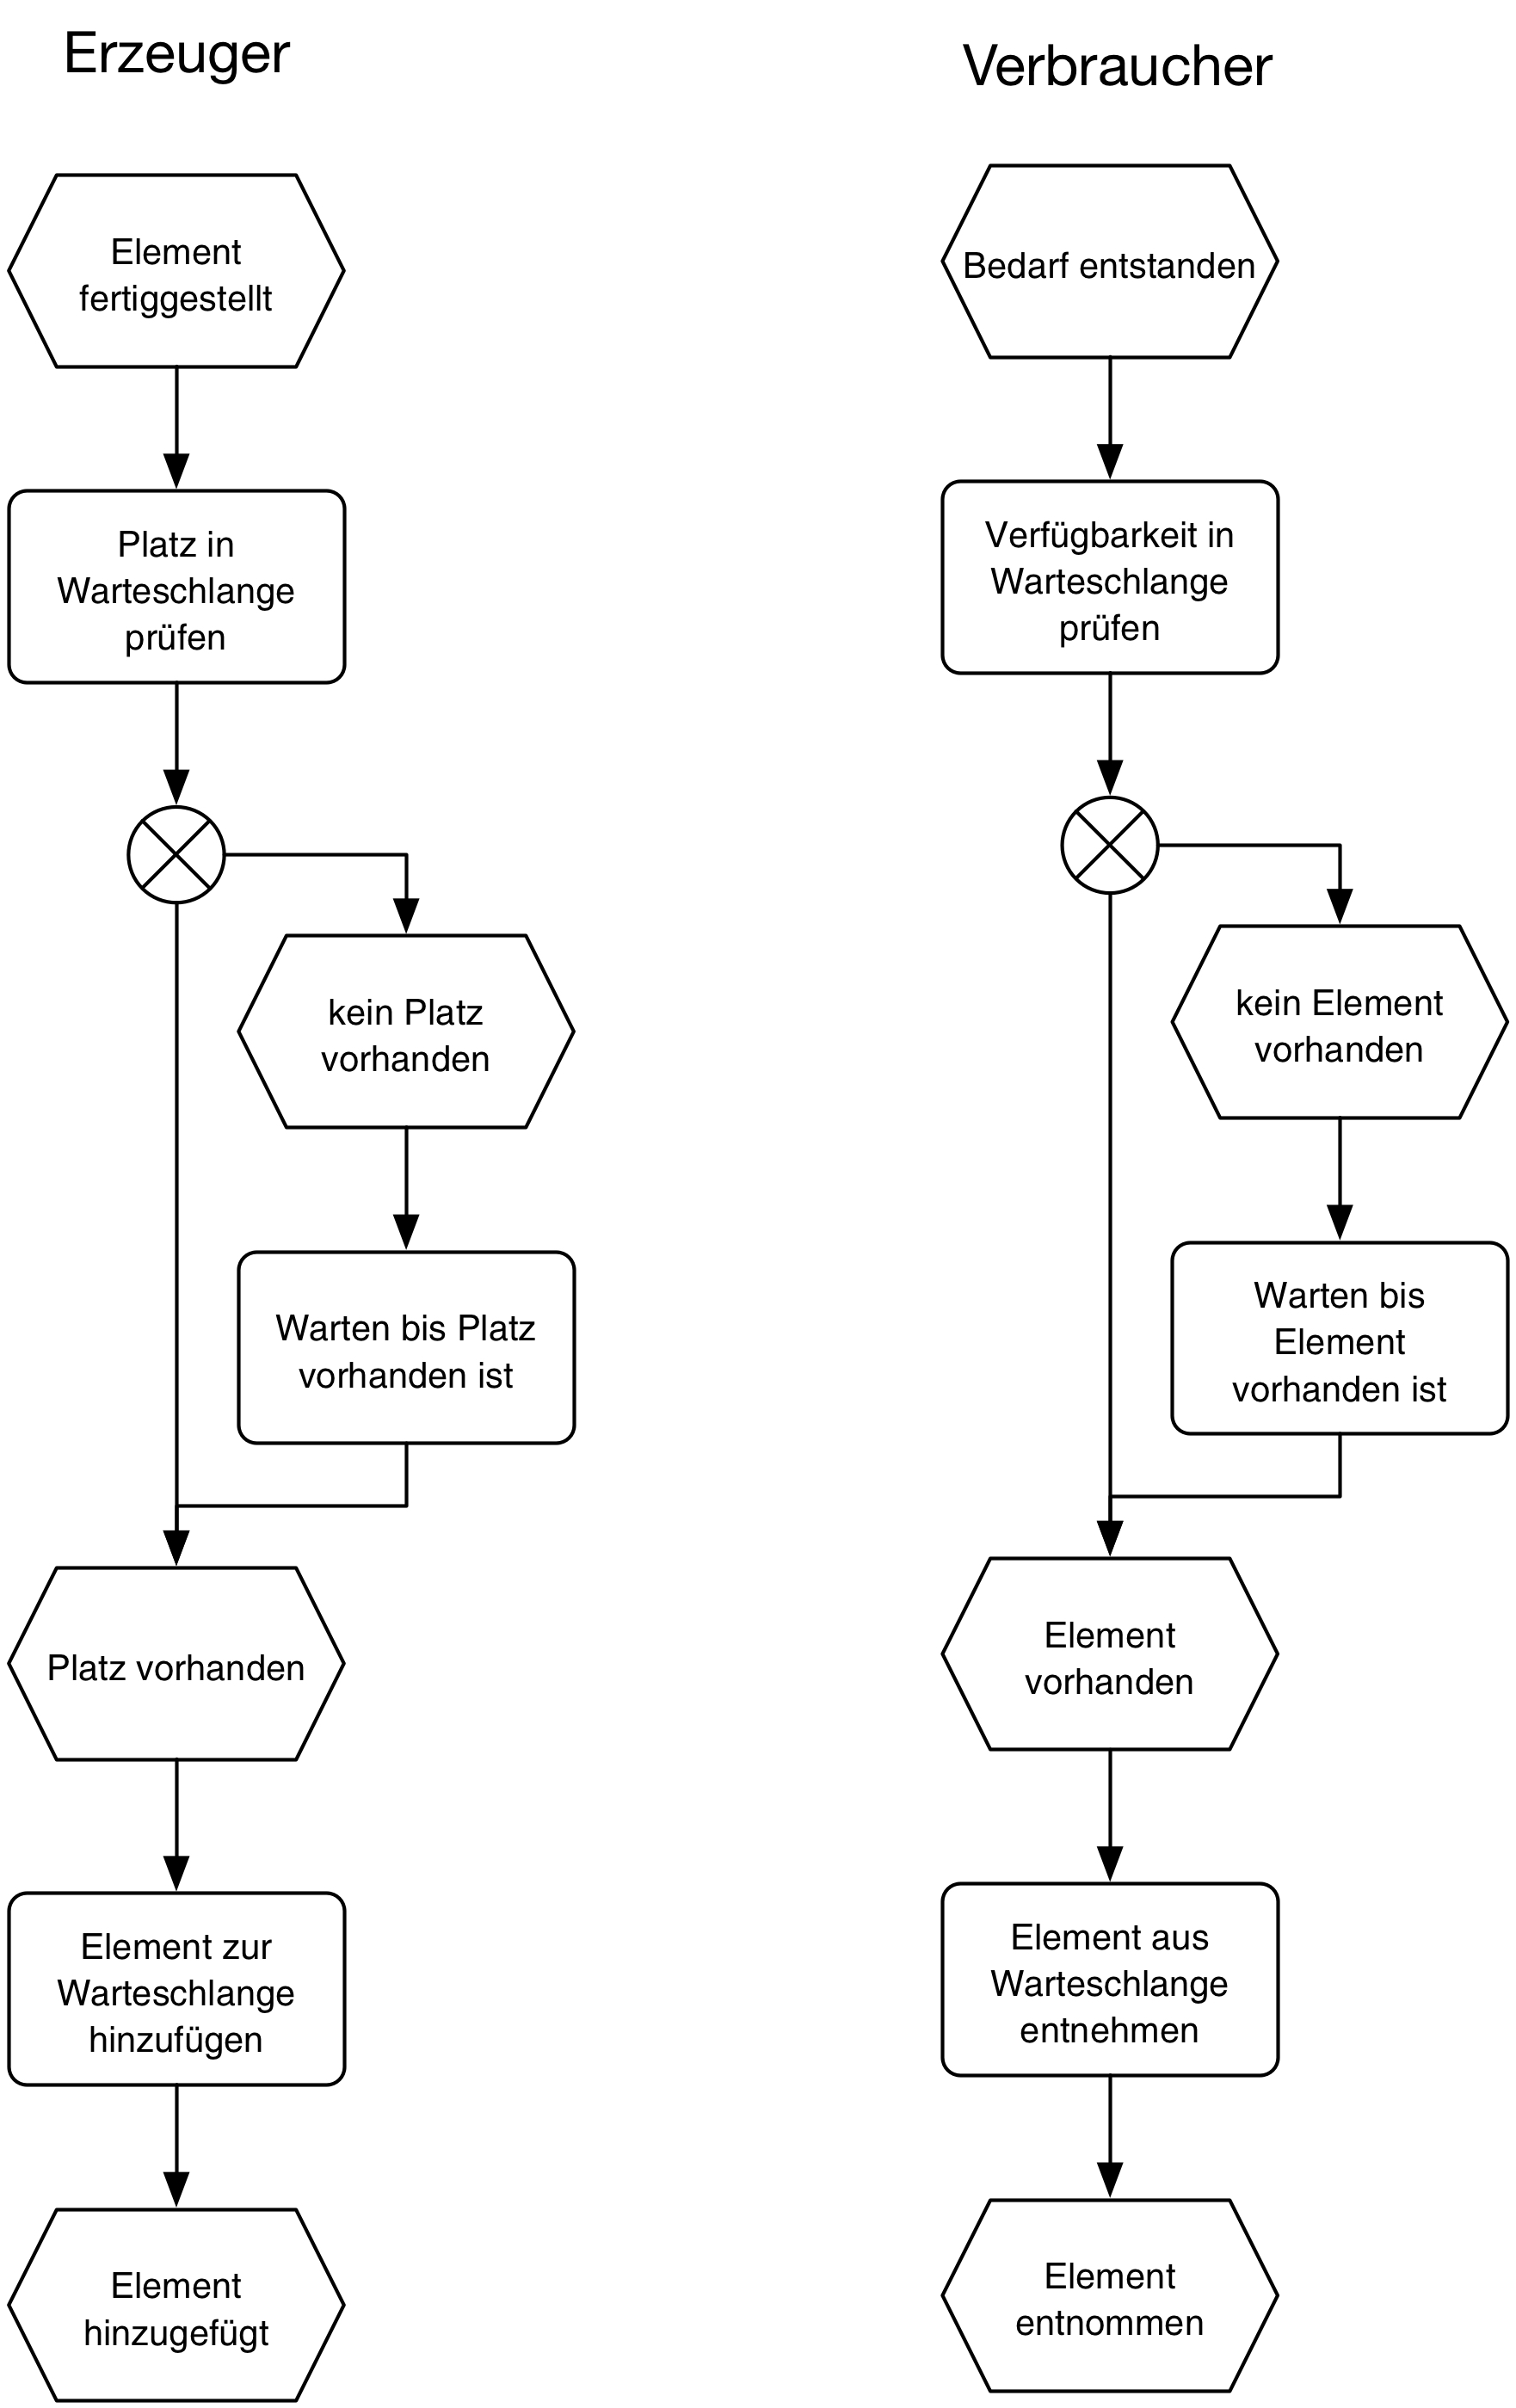
\includegraphics[width=.5\textwidth]{Erzeuger-Verbraucher-EPK.jpg}
\caption{Ereignisgesteuerte Prozessketten}
\label{fig:epk}
\end{center}
\end{figure}

% subsection ereignisgesteuerte_prozessketten (end)

\subsection{UML–Diagramm} % (fold)
\label{sub:uml_diagramm}
\begin{figure}[H]
\begin{center}
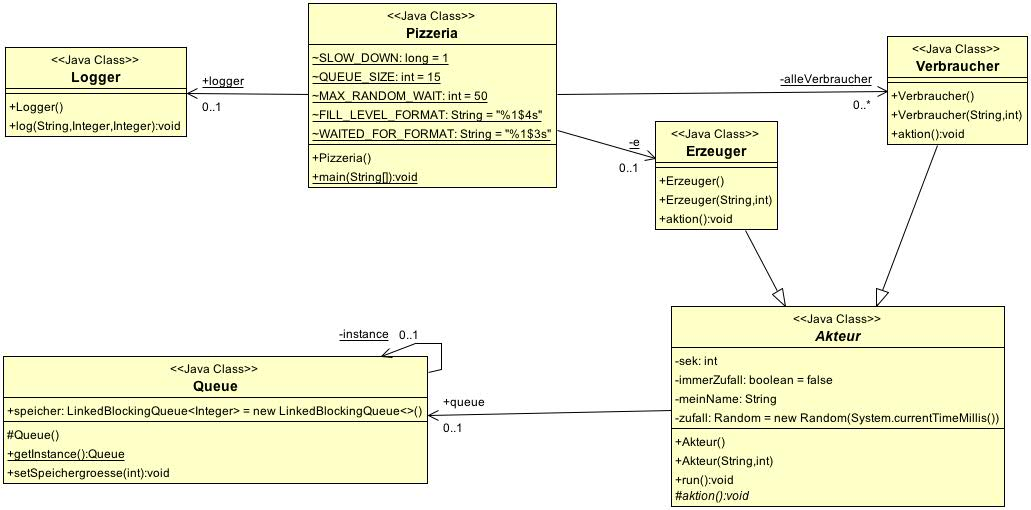
\includegraphics[width=\textwidth]{UML.jpg}
\caption{UML–Diagramm}
\label{fig:epk}
\end{center}
\end{figure}
% subsection uml_diagramm (end)

% section modellierung (end)

\newpage
\section{Implementierung} % (fold)
\label{sec:implementierung}

\subsection{Klasse: Akteur} % (fold)
\label{sub:klasse_akteur}
In der der abstrakten Klasse \code{Akteur} werden die Eigenschaften und Methoden zusammengefasst, die den Klassen \code{Erzeuger} und \code{Verbraucher} gemeinsam sind. Dazu gehören die Angaben zur Wartezeit \code{sek} bzw. \code{immerZufall} sowie die Bezeichnung \code{meinName}, die bei der Ausgabe dazu dienen kann, die Akteure zu unterscheiden. Diese Variablen werden von den Konstruktoren beim Erzeugen der Objekte befüllt. Des weiteren wird ein Generator für Pseude–Zufallszahlen sowie eine Referenz auf die Warteschlange benötigt.

In der Methode \code{run()}, die beim Starten des Threads aufgerufen wird, wird zunächst wie gefordert der Name und der Füllstand der Queue, ergänzt mit der Wartezeit ausgegeben. Anschließend wird die abstrakte Methode \code{aktion()} aufgerufen, welche die spezifischen Aktionen der abzuleitenden Klassen ausführt. Abschließend wird durch Aufruf der Methode \code{sleep()} der Elternklasse \code{Thread} die vorgegebene oder zufällig bestimmte Zeit gewartet.

Die Klasse \code{Akteur} implementiert keinen Zugriff auf die Queue und betritt somit keinen kritischen Abschnitt.
% subsection klasse_akteur (end)

\subsection{Klasse: Erzeuger} % (fold)
\label{sub:klasse_erzeuger}
Die von \code{Akteur} abgeleitete Klasse \code{Erzeuger} implementiert lediglich die Methode \code{aktion()}. Hierzu muss der kritische Abschnitt betreten werden. Hierin muss geprüft werden, ob Platz in der Queue vorhanden ist. Falls nicht, muss gewartet werden, bis dies der Fall ist. Wenn Platz vohanden ist, wird das produzierte Element\footnote{Hierbei handelt es sich in der Simulation um den Integerwert 1} in der Queue abgelegt. Anschließend wird der kritische Abschnitt wieder verlassen.

Diese Vorgehensweise entspricht der Implementierung der \code{put() } der Klasse \code{LinkedBlockingQueue}, welche indirekt über die Klasse \code{Queue} aufgerufen wird.\footnote{vgl. \cite{javadoc:lbqsourceput}}

Wie im Abschnitt~\myref{sub:kritische_abschnitte} ausgeführt, sind das Hinzufügen und das Entnehmen von ELementen bei \ac{FIFO} Warteschlangen getrennte kritische Abschnitte. Somit kann das Warten im Falle einer vollen Warteschlange durchgeführt werden, ohne eine Deadlock–Situation herbeizuführen.
% subsection klasse_erzeuger (end)

\subsection{Klasse: Verbraucher} % (fold)
\label{sub:klasse_verbraucher}
Die von \code{Akteur} abgeleitete Klasse \code{Verbraucher} implementiert lediglich die Methode \code{aktion()}. Hierzu muss der kritische Abschnitt betreten werden. Hierin muss geprüft werden, ob mindestens ein Element in der Queue vorhanden ist. Falls nicht, muss gewartet werden, bis dies der Fall ist. Wenn ein Element vohanden ist, wird das älteste entnommen. Anschließend wird der kritische Abschnitt wieder verlassen.

Diese Vorgehensweise entspricht der Implementierung der \code{take()} der Klasse \code{LinkedBlockingQueue} welche indirekt über die Klasse \code{Queue} aufgerufen wird.\footnote{vgl. \cite{javadoc:lbqsource}} 
% subsection klasse_verbraucher (end)

\subsection{Sonstige Programmmerkmale} % (fold)
\label{sub:sonstige_programmmerkmale}
Die Klasse \code{Queue} realisiert das Singleton–Entwurfsmuster, um ein Element der Klasse \code{LinkedBlockingQueue} der gewünschten Größe allen beteiligten Objekten und damit allen Threads zugänglich zu machen.\footnote{vgl. \cite{gof}, Seite 127ff}

Die Klasse \code{Logger} übernimmt die geforderte Ausgabe von „E“ bzw. „V” gefolgt von der Angabe der Zahl der momentan in der Warteschlange vorhandenen Elementen. Ergänzt werden diese Angaben von der Wartezeit\footnote{Hierbei ist die Wartezeit innerhalb des kritischen Abschnitts nicht berücksichtigt} und der dem Verbraucher zugewiesenen laufenden Nummer. Durch die Ausgabe des kompletten, zuvor zusammengesetzten Ausgabestrings in einem einzigen Aufruf von \code{System.out.println()} wird hier der konkurrierende Zugriff auf die gemeinsame Resource der Bildschirmausgabe threadischer geregelt.\footnote{siehe auch Abschnitt~\myref{sub:realisierung_mit_linkedblockingqueue}}

Die Klasse Pizzeria stellt das Gerüst der Anwendung dar. Hierin werden neben einigen Konstanten auch die benötigten Obkekte der Klassen \code{Logger} und \code{Erzeuger} sowie eine \code{ArrayList} für die nach dem Programmstart zu bestimmende Anzahl der Verbraucher definiert. Die Wartezeiten für die Verbraucher und den Erzeuger werden abgefragt und die Threads erzeugt und gestartet. Anschließend werden alle weiteren Schritte des Programms in den Threads ausgeführt. 
% subsection sonstige_programmmerkmale (end)
% section implementierung (end)

\newpage
\section{Laufzeitbetrachtungen} % (fold)
\label{sec:laufzeitbetrachtungen}

\subsection{Erzeuger schneller als Verbraucher} % (fold)
\label{sub:erzeuger_schneller_als_verbraucher}

% subsection erzeuger_schneller_als_verbraucher (end)

\subsection{Erzeuger langsamer als Verbraucher} % (fold)
\label{sub:erzeuger_langsamer_als_verbraucher}

% subsection erzeuger_langsamer_als_verbraucher (end)

\subsection{Ezeuger und Verbraucher gleich schnell} % (fold)
\label{sub:ezeuger_und_verbraucher_gleich_schnell}

% subsection ezeuger_und_verbraucher_gleich_schnell (end)

\subsection{Reduzierung auf einen Erzeuger und einen Verbraucher} % (fold)
\label{sub:reduzierung_auf_einen_erzeuger_und_einen_verbraucher}

Facade–Designpattern: Die n Verbraucher mit zufälligen Wartezeiten verhalten sich wie 1 Verbraucher mit kürzeren, aber ebenfalls zufälligen Wartezeiten. Dadurch ist die Anzahl der Verbraucher und analog dazu auch die der Erzeuger für die Betrachtung irrelevant.

% subsection reduzierung_auf_einen_erzeuger_und_einen_verbraucher (end)

% section laufzeitbetrachtungen (end)
\addtocontents{toc}{\protect\newpage}
\section{Fazit \& Ausblick} % (fold)
\label{sec:fazit_ausblick}

\subsection{Fazit} % (fold)
\label{sub:fazit}
Die vorliegende Arbeit gibt einen ersten Einblick in die behandelten Themanfelder „Erzeuger–Verbraucher–Problem“ und „Threading“. Die hierzu benötigten Konzepte sowie die von der Java–Umgebung zur Verfügung gestellten Werkzeuge zur Threadprogrammierung und Synchronisation wurden in Kapitel~\ref{sec:erzeuger_und_verbraucher} erläutert, bevor in Kapitel~\ref{sec:modellierung} die Anwendung entsprechend den Spezifikationen entworfen und implementiert wurde. Verschiedene Programmläufe wurden beobachtet, beschrieben und bewertet.

% subsection fazit (end)

\subsection{Ausblick} % (fold)
\label{sub:ausblick}
Weitere Entwicklungsmöglichkeiten bestehen im Ausbau der Anwendung, um verschiedene Szenarien simulieren zu können. So können z.B. Erzeuger mit variablen Arbeitsgeschwindigkeiten (höhere Belastung von Maschinen oder Menschen), zusätzlichen Erzeugern (Wie lange dauert das Anfahren?), Hinterlegung von Kosten für Lagerhaltung, Wartezeiten bei Erzeuger oder Verbraucher, etc. Bis hin zu hinterlegter Kalkulation, das den Endpreis des Produktes ermittelt und somit steuernd auf die Nachfrage einwirkt.
Hierdurch könnten Aussagen zu Stoßzeiten (Gastronomie, Einzelhandel, Energie, Webserver, ...) getroffen werden. 

Für eine solche feingliedrige Simulation ist eine eigene Implementierung der Queue oder evt. sogar des Threading denkbar, um an beliebigen Stellen den Zustand des Systems abfegen und analysieren zu können.

Ebenfalls kann in einer weiteren Arbeit untersucht werden, wie häufig ein Fehler, wie er in Abschnitt~\myref{sub:korrektes_logging} beschrieben ist vorkommt. Die Anwendung könnte dann bei Bedarf entlang der beschriebenen Lösungskonzepte erweitert bzw. neu implementiert werden.
% subsection ausblick (end)

% section fazit_ausblick (end)
%!TEX root = /Users/stwaidele/Dropbox (Leisinger)/02 - AKAD/Projektbericht/Möglichkeiten der Digitalen Kontaktaufnahme im Endkundenbereich/vorlage.tex

\appendix

\section{Quelltext der Anwendung} % (fold)
\label{sec:quelltext_der_anwendung}

% section quelltext_der_anwendung (end)

\section{Ergebnisse verschiedenener Programmläufe} % (fold)
\label{sec:ergebnisse_verschiedenener_programmlaufe}

% section ergebnisse_verschiedenener_programmlaufe (end)

\end{spacing}

\clearpage

% Literaturverzeichniss - Ab hier wieder Roemische Seitenzahlen
\pagestyle{plain}
\pagenumbering{roman}
\setcounter{page}{\theromanPagenumber}
%\addcontentsline{toc}{section}{Literatur-- und Quellenverzeichnis}
\renewcommand{\refname}{Literatur-- und Quellenverzeichnis}
%\bibliographystyle{alpha}
% http://blog.lewumpy.de/2011/01/latex-vorlage-fur-deutsches-literaturverzeichnis-und-zitierstil/
\bibliographystyle{mlu_ifg}
\bibliography{jav02-literatur}
\onehalfspacing
\clearpage

\pagestyle{empty} 
\thispagestyle{empty}

\begin{center}
{\Large Eidesstattliche Erklärung}
\vspace*{4cm}\end{center}
\noindent
Ich versichere, dass ich das beiliegende Assignment selbstständig verfasst, keine anderen als die angegebenen Quellen und Hilfsmittel benutzt sowie alle wörtlich oder sinngemäß übernommenen Stellen in der Arbeit gekennzeichnet habe. 
\vspace{3cm}

\rule[0.5ex]{6.5cm}{1pt}
\hfill
\rule[0.5ex]{6.5cm}{1pt}
\\(Datum, Ort)
\hfill
(Unterschrift)


\end{document}

